\section{Ejemplo de procedimiento PID}\label{Ap:control}

A continuación, se presentará el procedimiento para la realización del control PID que se llevará a cabo.  

En un primer momento, se realiza la comunicación entre Arduino y simulink (Figura \ref{fg:Comunicacion}) para obtener las mediciones del sensor, es importante señalar, que se toma en cuenta la pendiente de operación del sensor para poder procesar los datos en simulink.

\begin{figure}[h!]
            \centering
            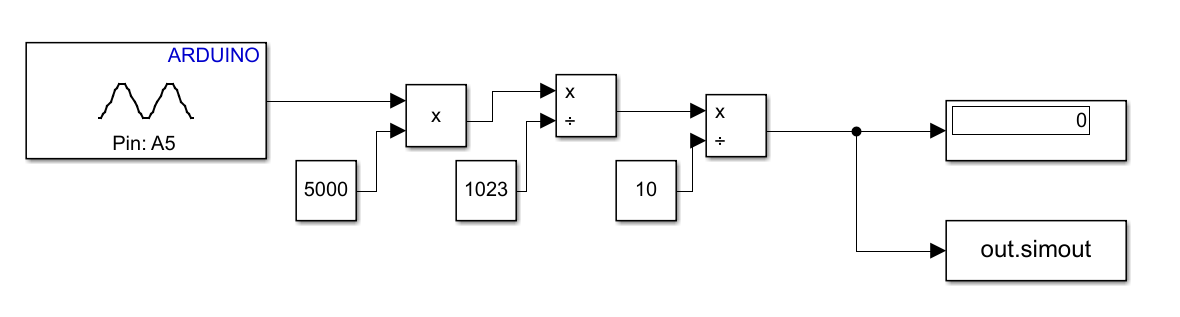
\includegraphics[scale=0.4]{images/Capitulo 3/3.1.2/comunicacion.png}
            \caption{Comunicación Simulink-Arduino}
            \label{fg:Comunicacion}
        \end{figure}
Una vez que la comunicación se realizó de manera correcta, se podrá ver en simulink la curva de calentamiento del sensor, es importante establecer un tiempo que sea los suficientemente largo para observar la estabilización del valor máximo que se alcanza.
En este caso se observa como parte de la temperatura ambiental y aumenta la temperatura, presentando un comportamiento logarítmico (Figura \ref{fg:Curva_calent}), este comportamiento corresponde a un sensor LM35 sin embargo, se espera un comportamiento similar en otros sensores como el DS18B20.

\begin{figure}[h!]
            \centering
            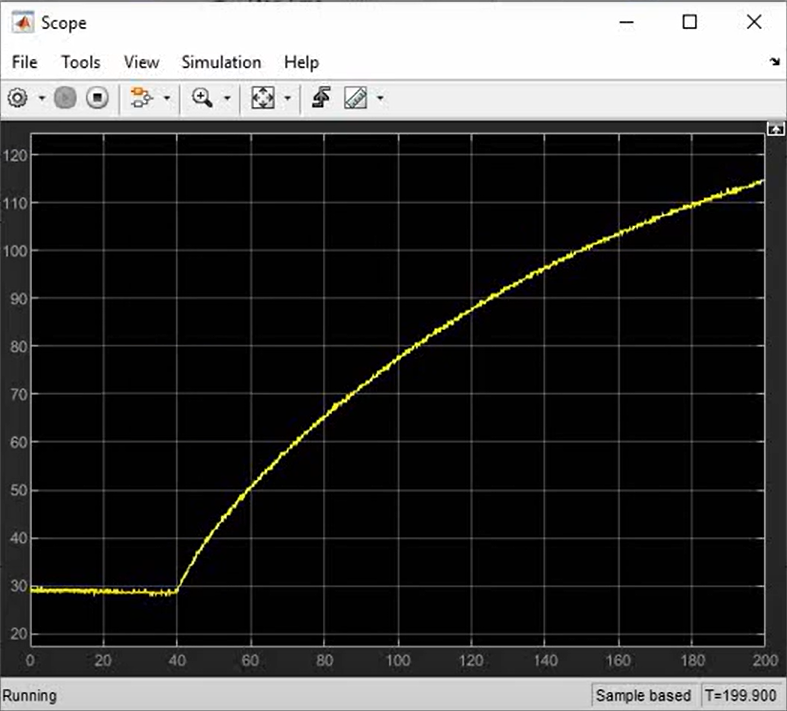
\includegraphics[scale=0.4]{images/Capitulo 3/3.1.2/curva_calentamiento.png}
            \caption{Curva de calentamiento LM35}
            \label{fg:Curva_calent}
        \end{figure}
Con las mediciones realizadas, se procede a obtener la función de transferencia del sistema (Figura \ref{fg:Func_transfer}).

\begin{figure}[h!]
            \centering
            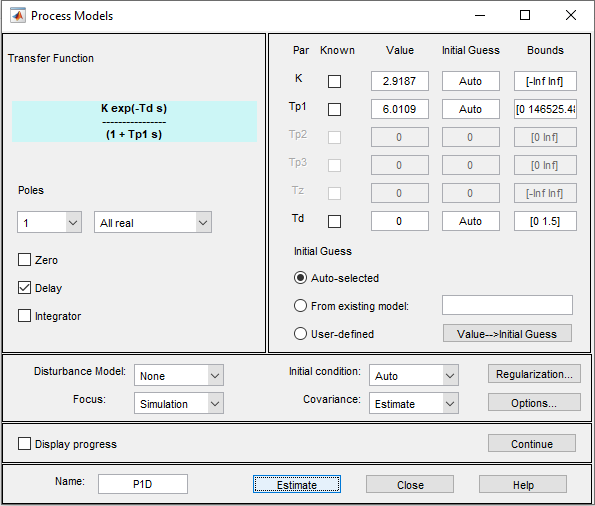
\includegraphics[scale=0.5]{images/Capitulo 3/3.1.2/Ftransferencia.png}
            \caption{Función de transferencia obtenida con Simulink}
            \label{fg:Func_transfer}
        \end{figure}
        
        
Se agrega el PID a la comunicación de Simulink y Arduino (Figura \ref{fg:PID+CSA}) y se ajusta la señal para que el control de comporte de la manera deseada, evitando un sobre impulso o que el sistema tarde demasiado en llegar al valor requerido (Figura \ref{fg:PIDTS}).

\begin{figure}[h!]
            \centering
            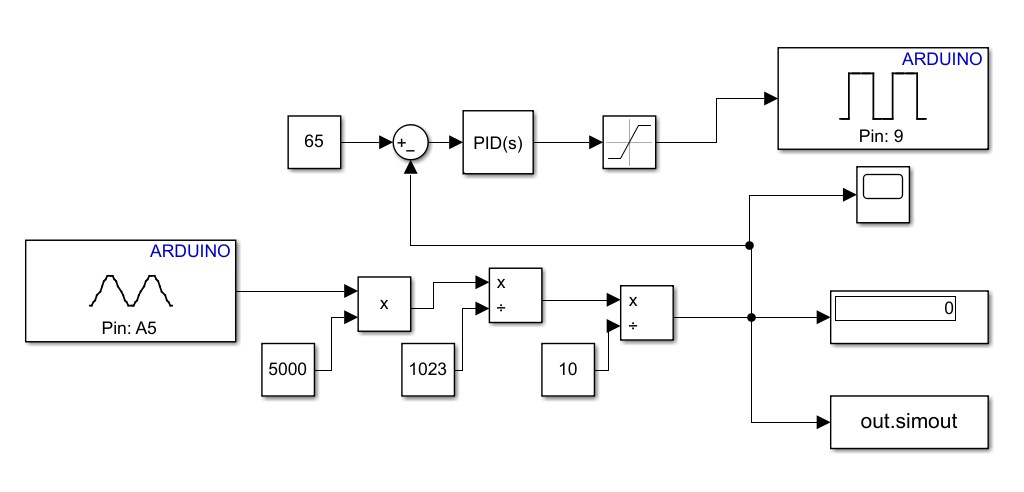
\includegraphics[scale=0.3]{images/Capitulo 3/3.1.2/ControlPID_comSimu.png}
            \caption{Control PID y comunicación Simulink-Arduino}
            \label{fg:PID+CSA}
        \end{figure}

\begin{figure}[h!]
            \centering
            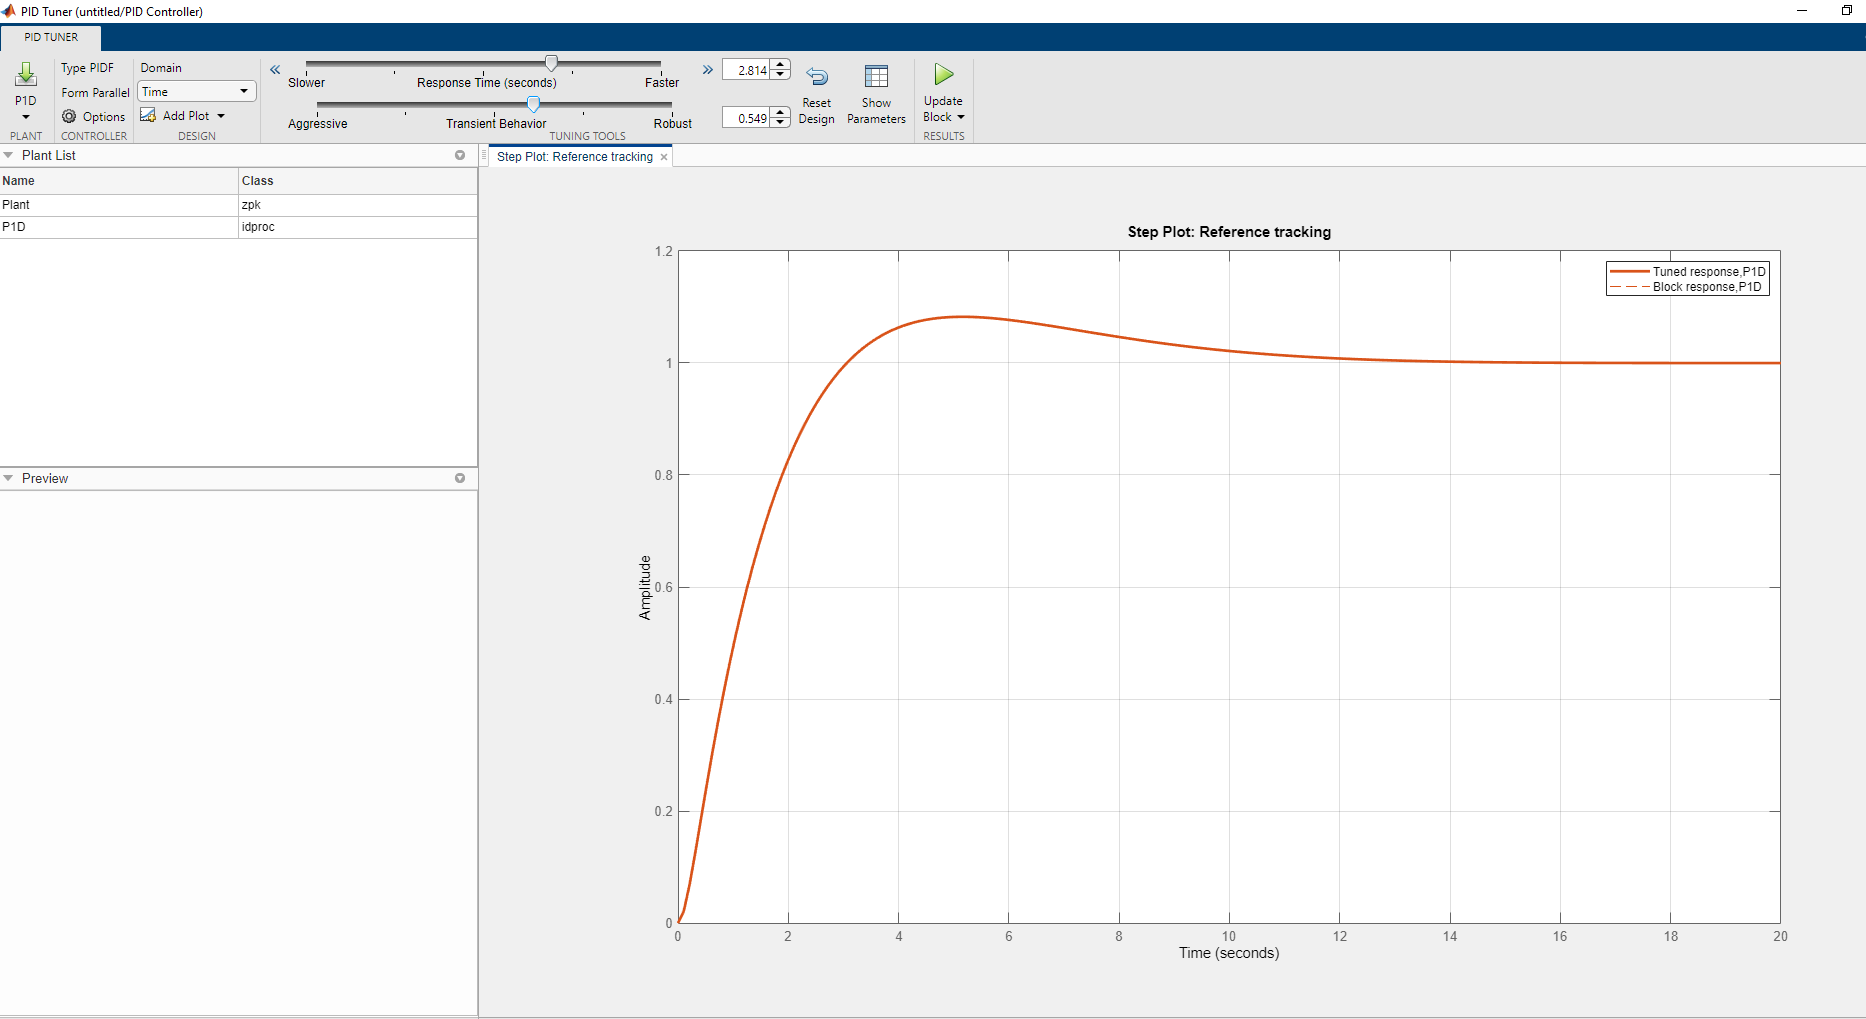
\includegraphics[scale=0.25]{images/Capitulo 3/3.1.2/PID_Tuner.png}
            \caption{PID Tuner Simulink}
            \label{fg:PIDTS}
        \end{figure}
        